\documentclass[spanish]{article}
\usepackage[utf8]{inputenc}
\usepackage{babel}
\usepackage{multirow}
\usepackage{graphicx}
\usepackage{float}
\usepackage{enumerate}
\usepackage{lmodern}
\usepackage[T1]{fontenc}
\usepackage{mathtools}
\usepackage[usenames,dvipsnames]{xcolor}
\usepackage{graphicx}
\usepackage{lscape} 
\usepackage{pdflscape} 
\usepackage{fancyvrb}
\usepackage{listings}
\usepackage{fancybox}
\usepackage{listings}
\definecolor{light-gray}{gray}{0.85}
\definecolor{mimalva}{rgb}{0.58,0,0.99}

    \lstset{
	basicstyle=\normalsize\ttfamily,     
	numbers=left,               
	language=c,
	stepnumber=1,               
	numbersep=1em,              
	aboveskip=1em,
	keepspaces=false,      
	showstringspaces=false,        
	belowskip=0.2em,
	keywordstyle=\ttfamily\color{ForestGreen}\bfseries,
		stringstyle=\color{RubineRed}, 
        %identifierstyle=\ttfamily\color{Sepia}\bfseries,
        commentstyle=\color{NavyBlue},
        morecomment=[l][\color{Periwinkle}]{\#},
	backgroundcolor=\color{white},
	numberstyle=\footnotesize\color{Gray},
	frame=single,
	rulecolor=\color{NavyBlue},
    }

\title{Titulo Plantilla \\ Mas titulo \\ Asignatura}

\author{Nombre Apellido}

%si quieres quitar la fecha descomentas la linea de abajo
%\date{}

\begin{document}

%\begin{figure}
%  \centering
%    
\includegraphics[width=0.99\textwidth]{Logo_computacion}
%\end{figure}

\maketitle

\section{Primera Seccion}
	puedo tener subsecciones
		\subsection{Primera Sección}
		y mas subsecciones	
			\subsubsection{Segunda Sección}
			algo por aquí


\section{Lista con Viñetas}

	 \begin{itemize}
	 
		\item 1er Item 	 
	 	\item 2do Item 	 
	 	\item 3er Item 	 
	 	\item 4to Item 	 
	 \end{itemize}

\section{Lista con Números}

	 \begin{enumerate}
		\item  Item 	 
	 	\item  Item 	 
	 	\item  Item 	 
	 	\item  Item 	 
	 \end{enumerate}

\section{Lista con Viñetas Anidadas}

	 \begin{itemize}
	 
		\item 1er Item 	 
			 \begin{itemize}
			 	\item 1.1 Item 	 
	 	     	\item 1.2 Item 	 
	   	     	\item 1.3 Item 	 
	 		 	\item 1.4 Item 	 
	 		 \end{itemize}
		
	 	\item 2do Item 	 
	 	\item 3er Item 	 
	 	\item 4to Item 	 
	 \end{itemize}
	 
	 
\section{Mostrar una imagen}

\begin{figure}[htb]
\centering
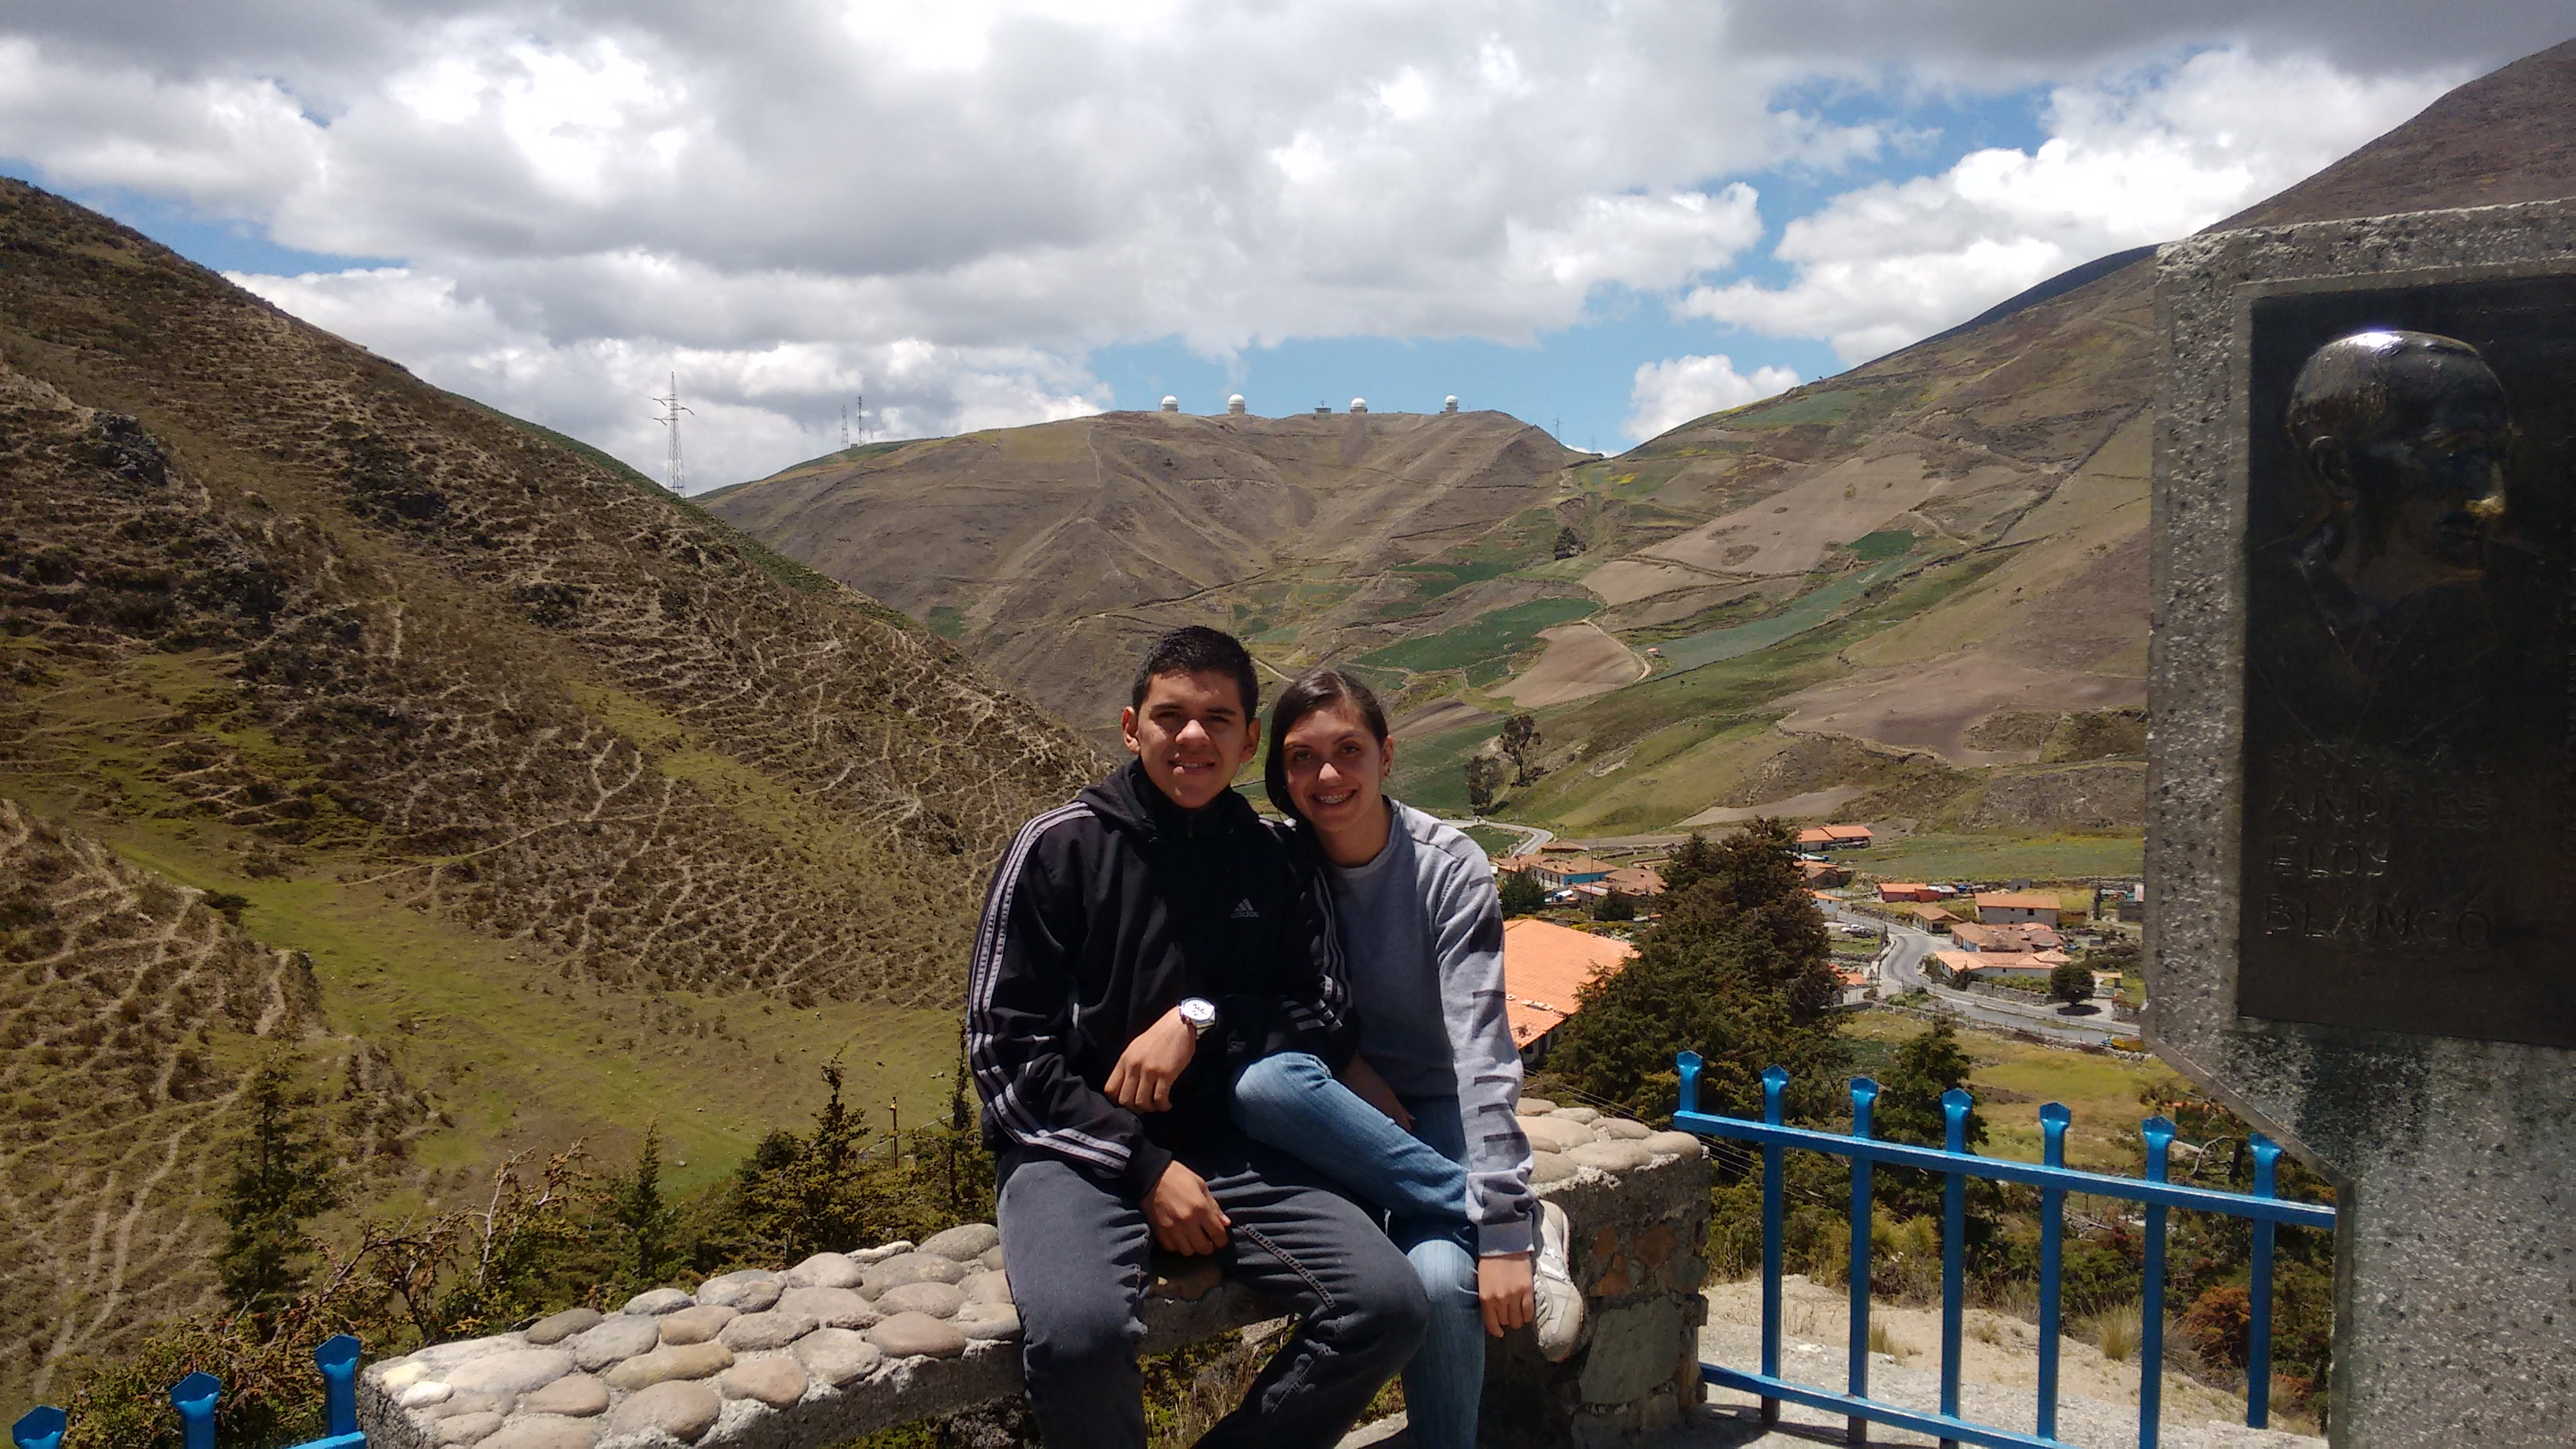
\includegraphics[width=0.70\textwidth]{foto.jpg}
\caption{Todo Estará Bien :)}
\label{i1}
\end{figure}	 

%para salto de pagina
\break 

\section{Matemáticas}

para $R_{1}$:
\begin{equation}\label{9}
V_{R1}(t) = V_{f} * \dfrac{R_{1}+R_{2} * e^{-t*\left(  \dfrac{R_{1} + R_{2}}{C*R_{1}*R_{2}} \right) } }{R_{1} +R_{2}}
\end{equation}

\begin{equation}\label{10}
i_{R1}(t) = \dfrac{V_{f}}{R_{1}} * \dfrac{R_{1}+R_{2} * e^{-t*\left(  \dfrac{R_{1} + R_{2}}{C*R_{1}*R_{2}} \right) } }{R_{1} +R_{2}}
\end{equation}

para $R_{2}$:
\begin{equation}\label{11}
V_{R2}(t) = V_{c}(t)
\end{equation}

\begin{equation}\label{12}
i_{R2}(t) = \dfrac{V_{f}}{R_{1} + R_{2}} - \dfrac{V_{f}}{R_{1} + R_{2}} * e^{-t*\left(  \dfrac{R_{1} + R_{2}}{C*R_{1}*R_{2}} \right)}
\end{equation}



Cabe destacar que las ecuaciones (\ref{9}),(\ref{10}),(\ref{11}),(\ref{12}) dependen de los valores de los resistores, el capacitador y la fuente. 

\section{Código}

\begin{lstlisting}
#include <stdio.h>
#include <stdlib.h>
#include <unistd.h>
#include <sys/types.h>
#include <sys/msg.h>
#include <errno.h>
#include <signal.h>
#include "colamsg.h"

void exit_signal(int);

void exit_signal(int num_signal)
{
  printf("\n\n\tHasta luego!\n");
  fflush(stdout);  
  exit(EXIT_SUCCESS);  
}

\end{lstlisting}

\end{document}
\grid
